\chapter{Technical specifications}
\label{chap:tech}
SALSA onsala is a modified television antenna with a diameter of 2.3~m and designed
to operate at 1420\,MHz.

\section{Angular resolution and accuracy}
\label{sect:ares}
SALSA has an angular resolution of about 6$^\circ$ (\emph{full width half
maximum}) at 1420\,MHz. This value has been measured using the Sun, see Fig.
\ref{fig:beam}. For comparision, remember that the full moon has an angular
diameter of about half a degree, or 30~minutes of arc. The motors track 
in steps of 0.125$^\circ$ around each axis, hence this is the telescope
accuracy in perfect conditions. However, if it is windy\footnote{You can check
the current wind speed at http://wx.oso.chalmers.se/weather/} the telescope
may wobble in the wind (around the wanted position) and hence disturb
the pointing of the telescope during small time intervals with 1-2$^\circ$. 
This should however not be a big concern for users since the wobbles are smaller
than the angular resolution.
\begin{figure}[ht]
\begin{center}
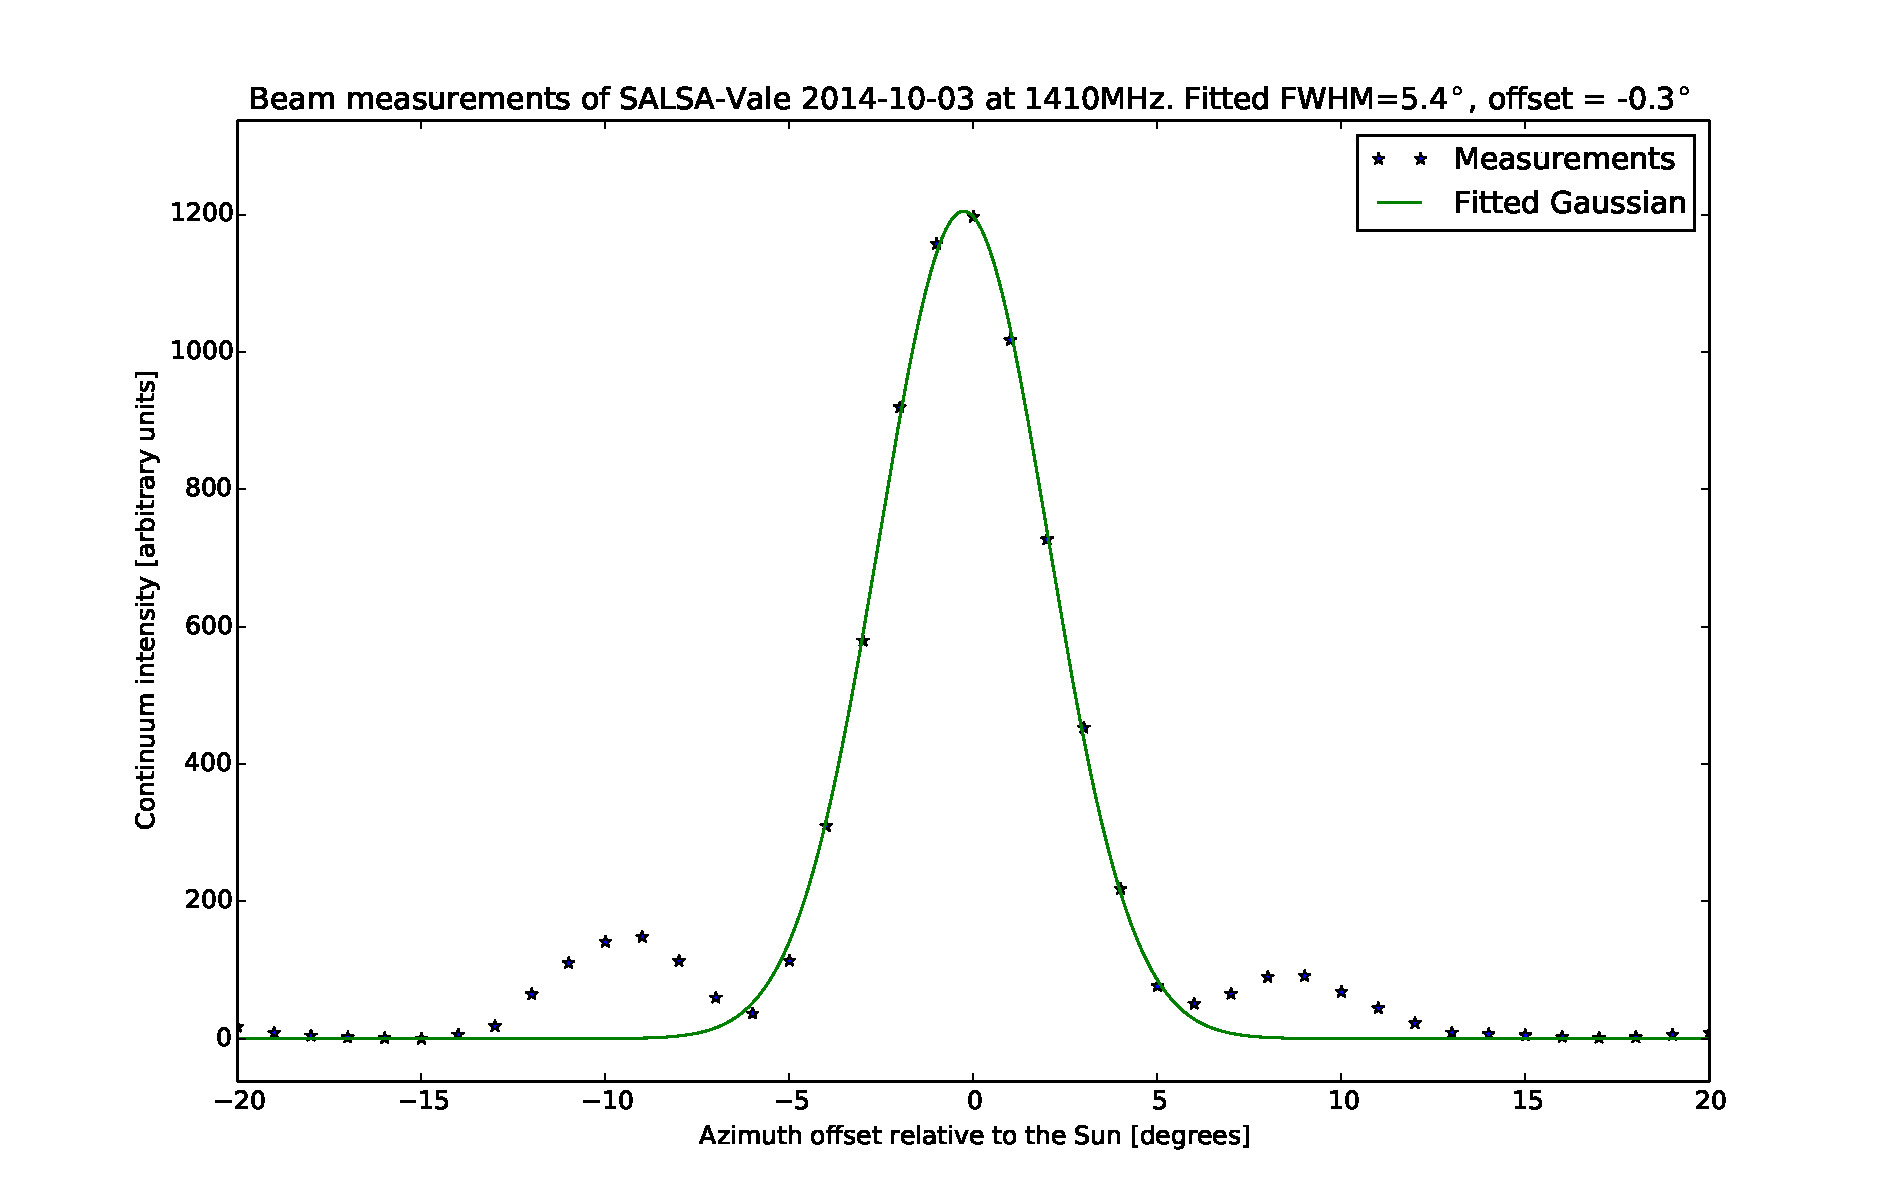
\includegraphics[width=\textwidth]{../figures/Beam_vale_2014-10-03.pdf}
\end{center}
\caption{The beam of Vale measured using the Sun at 1410\,MHz. A Gaussian fit
gives the FWHM=5.4$^\circ$. The sidelobes of the Sinc-function are clearly
visible, as expected for a circular aperture.}
\label{fig:beam}
\end{figure}

\section{Spectral resolution and accuracy}
The telescope uses the \emph{Universal Software Radio Peripheral} (USRP) to
record data. The USRP acts as a sampler which records a time stream to the hard
drive of the control computer. The channelisation, i.e. construction of the
spectrum, is done in software (FFT). This means that the number of channels
(spectral resolution) is not fixed, nor is the bandwidth. The spectral
resolution is limited by the free space and processing speed of the control
computer. Up to 10\,MHz bandwidth with 8192 channels have been tested, but for
most observations the standard settings of 2\,MHz bandwidth and 256 channels
are sufficient, i.e. a frequency resolution of 7.8\,kHz per channel. If a finer
resolution is needed, it may be selected from the \emph{Advanced} tab in the
\emph{Receiver control} part of the SALSA control program, but we cannot offer
support for these advanced modes yet.

\section{Flux calibration and uncertainty}
Currently SALSA is NOT ACCURATELY FLUX CALIBRATED. This means that SALSA should
only be used to measure HI velocities, and not HI antenna temperatures. We aim
to make SALSA well calibrated in the future, but the system is still undergoing
changes which makes it unpractical to calibrate at this point. When the system
is well calibrated, this manual will be updated with that information.
